\chapter{Fundamentals}
\label{chap:refs}

Under the term \emph{ray tracing} we understand the utilization of algorithms that involve the casting of virtual light rays for generating images. The purpose of these light rays is to archive high visual realism by approximating real-life behavior \todo{is that right?}. The reason we are able to perceive nearby objects or persons is due to the fact that light, which is being emitted from light sources, either natural or artificial, is interacting with these objects or persons, it is being reflected off by their surfaces towards our vision sensory organs after possibly being reflected a multiple times before from other surfaces. \todo{what?}
The purpose of ray tracing algorithms is to imitate this behavior, usually by tracing these light rays in reverse order from the sensory organs (or a virtual camera or an "eye point") back to the emitting light source.

\begin{figure}[h]
	\centering
	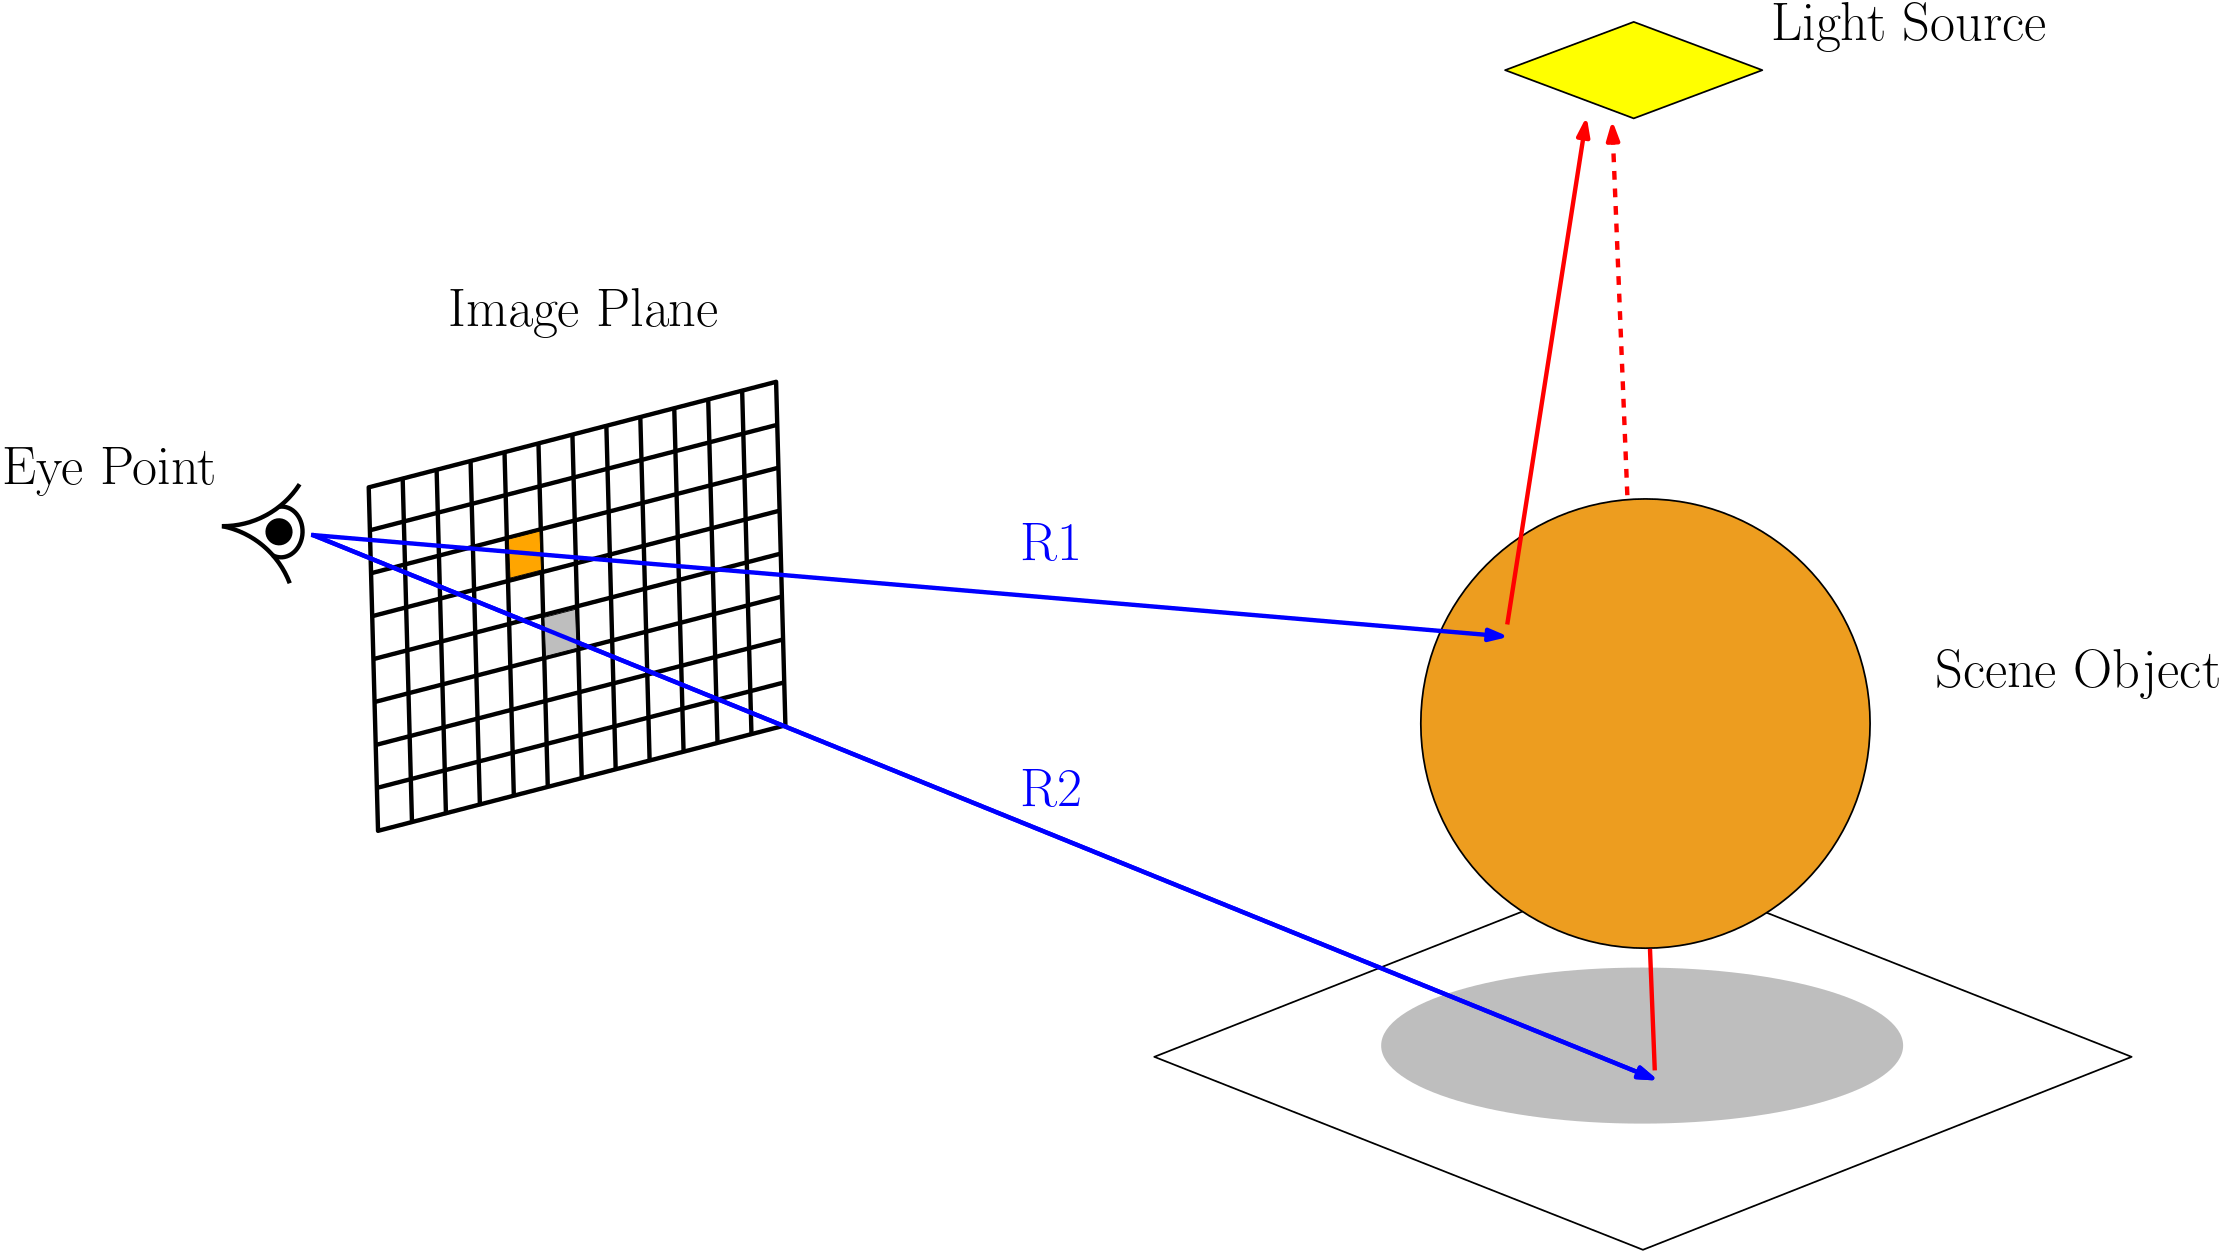
\includegraphics[width=.9\linewidth]{img/1 fundamentals/ray_tracing.png}
	\caption{Ray tracing procedure for calculating global illuminate.}
	\label{fig:raytracer_general}
\end{figure}

An advantage of these ray tracing algorithms is that the core procedure is straightforward when viewed from a theoretical point of view. Figure \ref{fig:raytracer_general} shows an example of a virtual scene. It consists of an orange sphere, a white ground plane, and a plane acting as an area light source. Furthermore, there exists an image plane on which the 2D image of the 3D scene will be projected. A ray is consisting of two components, an origin point and a direction vector. The "Eye Point" in \ref{fig:raytracer_general} will serve as the origin of the cast rays (sometimes, the Eye Point is referred to as Camera or Virtual Camera). In the figure, the image plane is composed of multiple quadratic "cells" that represent the actual pixels of the resulting image. Through each of these cells, a ray is cast into the scene from the eye point. The next step is to determine, whether that ray hit a particular geometry by performing intersection tests on all geometries in the scene. In case a geometry is hit, a secondary ray is generated with its origin at the intersection point and its direction toward the light source. In case this secondary light ray does not intersect any other geometry between its origin and the light source, this means that the first intersection point is exposed to light and the material color at that point is used for the corresponding pixel (see R1 in figure \ref{fig:raytracer_general}). Otherwise, the intersection point must be in shadow (see R2). This procedure generates an image with local illumination.

The following chapter is dedicated to providing background information on ray tracing, shape representation in rendering systems, and ray acceleration data structures. Furthermore, the Embree framework is introduced. \todo{maybe rephrase}

\section{Overview of Ray Tracing Algorithms}


\subsection{Origins of Ray Tracing}
As briefly mentioned in the Introduction, ray tracing was pioneered in 1968 by \cite{appel1968some}. The aim of his work was to provide basic shading for line drawings yielding a better communication of spatial relation and depth of objects in the rendered image.

\begin{figure}[h]
	\centering
	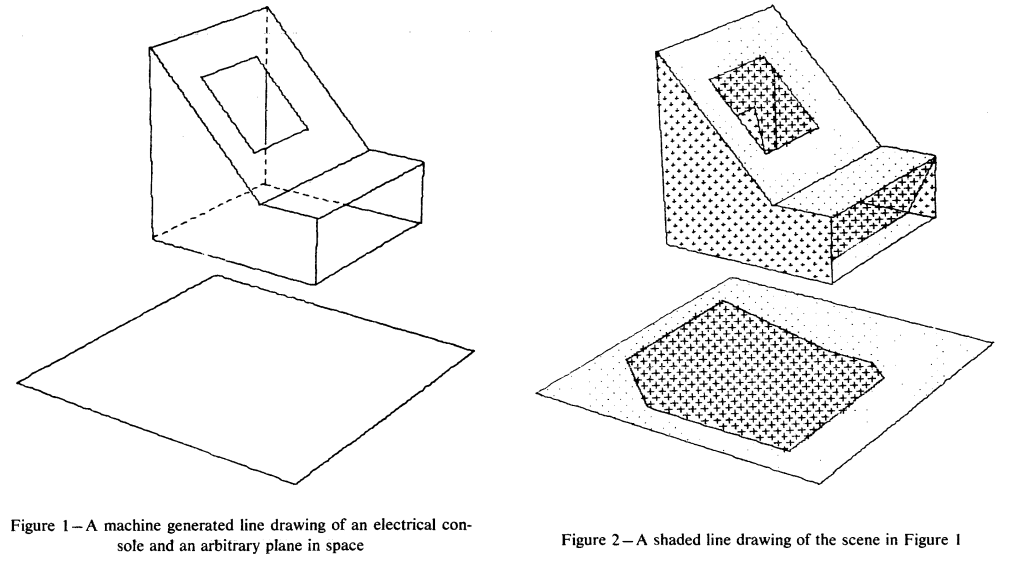
\includegraphics[width=1\linewidth]{img/1 fundamentals/appel_comp}
	\caption{Figures from \cite{appel1968some}. Left figure shows plain solid geometry and right figure shows the same solid with shading applied to it.}
	\label{fig:appel}
\end{figure}
\todo{can I use figures from other papers?}

Figure \ref{fig:appel} demonstrates this: without the additional shading information, it would be difficult for the observer to perceive the position of the upper geometry relative to the plane.

In order to achieve this shading, virtual light rays are shot from a scene light source in random directions. Whenever one such ray intersects a geometry, a character or symbol (e.g. a "plus"-symbol or small square) is placed at that intersection point. If enough such rays would be cast, areas on the solid that are exposed to light would be shaded by these symbols.
The result would then come to be by inverting the shaded and non-shaded areas of the geometry.

The intensity of light $I$ incident to the light source is described by the following equation:

\begin{equation}
I = S\frac{\cos{\theta}}{{D}^2}
\end{equation}

where $S$ is the intensity of the light source, $\cos{\theta}$ the angle between the ray and the surface normal at the intersection point and $D$ the distance between intersection point and light source.

In order to achieve convincing results, a high number of rays had to be generated ("Even for about 1000 light rays results were splotchy." \cite[p 3]{appel1968some}). At the time of publication, computational power of hardware could hardly be used for this.

The idea of casting rays later became a key utilization for a shading model that aimed for higher realism by taking the "global setting" of geometries into account \cite{whitted1979improved}. A variety of shading models existed at that time, which were able to convincingly display optical effects. However, these models usually worked only in special cases and not well with each other, as noted by Andrew Glassner in the preface of his book \citetitle{glassner1989introduction} \cite{glassner1989introduction}. \todo{is this good?} Some models existed that were good at calculating reflection effects, but could not handle refraction effects well. And vice versa. 

\cite{whitted1979improved} introduced a shading model that would truthfully simulate reflection, shadows and refraction as well as the effects of other conventional shading models at that time.  

The model builds upon an empirical reflection model devised by \cite{phong1975illumination}, which assumes that light is reflected from a surface is composed by three types of reflection: ambient reflection, diffuse reflection and specular reflection. It is given by the following equation:

\begin{equation} \label{eq:phong}
I = k_{a} + k_{d}\sum_{j}(n*L_{j}) + k_{s}\sum_{j}(n*L_{j}\prime)^{gl}
\end{equation}

\noindent where
\begin{description}
	\setlength\itemsep{0.05em}
	\item  [$I$] is the reflected intensity
	\item  [$I_{a}$] is the ambient reflection coefficient
	\item  [$k_{d}$] is the diffuse reflection coefficient
	\item  [$k_{s}$] is the specular reflection coefficient
	\item  [$n$] is the unit surface normal at an intersection point
	\item  [$L_{j}$] is a vector in the direction of the $j$th light source
	\item  [$L_{j}\prime$] is a half vector between the eye point and the $j$th light source, and
	\item  [$gl$] is the glossiness coefficient.
\end{description}

One limitation of this model is the assumption that the light sources are located at an infinite distance from the scene geometry, and thus, the model does not account for objects within the scene acting as light sources. It was observed in \cite{newell1977progression}, that this can critiacaly affect the specular reflection component of Equation \ref{eq:phong}.

As opposed the the Phong shading model, Whitted's model assumes that the light intensity $I$ arriving at the eye point from the intersection point $x$ is conglomerated by the specular reflection $S$ and transmission, $T$ as shown in Figure \ref{fig:whitted_model}.

\begin{figure}[h]
	\centering
	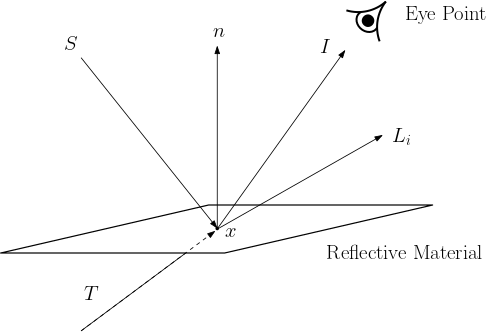
\includegraphics[width=.7\linewidth]{img/1 fundamentals/whitted.png}
	\caption{The light intensity $I$ arriving at the $Eye Point$ from a point $x$ on the surface is assumed to be composed of a specular component $S$ and a transmissive component $T$.}
	\label{fig:whitted_model}
\end{figure}


The model is given by the equation:
\begin{equation}
I = k_{a} + k_{d}\sum_{j}(n*L_{j}) + k_{s}S + k_{t}T
\end{equation}

\noindent where
\begin{description}
	\setlength\itemsep{0.05em}
	\item  $S$ is the light intensity of the specular reflection
	\item  $T$ is the light intensity of the transmissive reflection, and
	\item  $k_{s}$ is the transmission coefficien
\end{description}

The ambient and diffuse term are maintained from Equation \ref{eq:phong}. 
This model approximates the 

\begin{figure}
	\centering
	\subfloat[Light is reflected from other surfaces before reaching the Eye Point.]{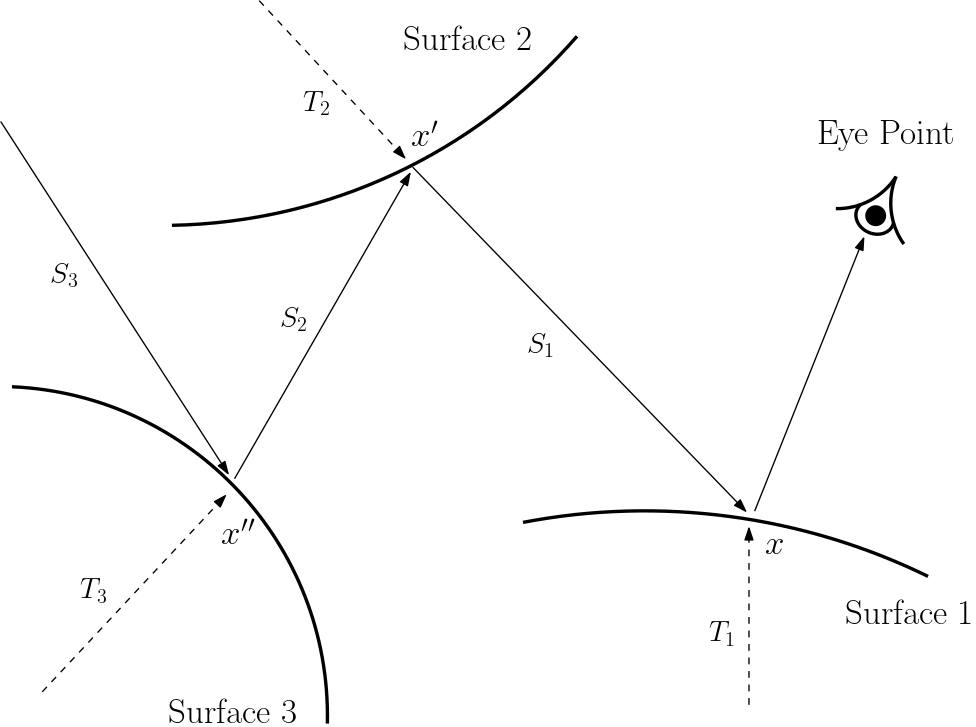
\includegraphics[width=.5\textwidth]{img/1 fundamentals/whitted_rays.png}\label{fig:whitted_rays}}
	\hfill
	\subfloat[Tree structure storing the individual reflection and transmission rays.]{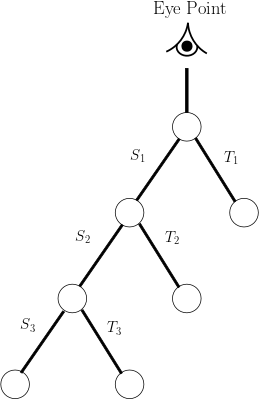
\includegraphics[width=.25\textwidth]{img/1 fundamentals/whitted_tree.png}\label{fig:whitted_tree}}
	\caption{Figures from the paper \citetitle{whitted1979improved} \cite{whitted1979improved}}
\end{figure}



\begin{figure}
	\centering
	\subfloat[Light is reflected from other surfaces before reaching the Eye Point.]{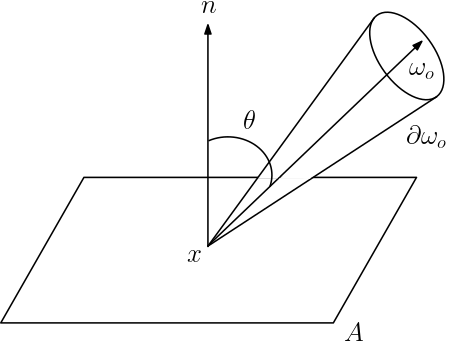
\includegraphics[width=.4\textwidth]{img/1 fundamentals/radiance.png}\label{fig:radiance}}
	\hfill
	\subfloat[Tree structure storing the individual reflection and transmission rays.]{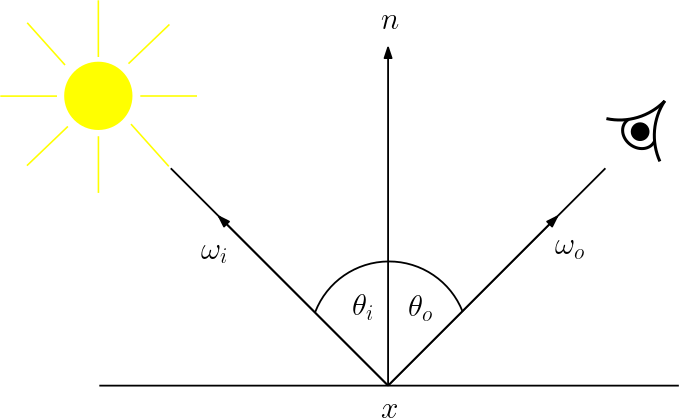
\includegraphics[width=.5\textwidth]{img/1 fundamentals/brdf.png}\label{fig:brdf}}
	\caption{Figures from the paper \citetitle{whitted1979improved} \cite{whitted1979improved}}
\end{figure}

\subsection{Path Tracing}


\begin{equation}
L(\omega_{o}) = \frac{\partial^2\phi}{\partial\omega_{o}\partial A\cos\theta}
\end{equation}

\noindent where
\begin{description}
	\setlength\itemsep{0.05em}
	\item  $\omega_{o}$ is the outgoing direction
	\item  $\phi$ is flux or radiance per unit time
	\item  $A$ is the surface area
\end{description}


\begin{equation}
BRDF(\omega_{i} \rightarrow \omega_{o}) = \frac{\partial L_{r}(\omega_{o})}{L_{i}(\omega_{i})\partial A\cos\theta}
\end{equation}

\noindent where
\begin{description}
	\setlength\itemsep{0.05em}
	\item  $L_r(\omega_{o})$ is the reflected radiance
	\item  $L_i(\omega_{i})$ is the incident radiance
\end{description}

\begin{equation}
L_{r}(\omega_{o}) = \int_{H(x)} L_{i}(\omega_{i})  BRDF(\omega_{i} \rightarrow \omega_{o}) \cos\theta\partial\omega_{i}
\end{equation}

\noindent where
\begin{description}
	\setlength\itemsep{0.05em}
	\item  $H(x)$ is a hemisphere over the interaction point $x$
\end{description}

\begin{equation}
L(\omega_{o}) = L_{e}(\omega_{o}) \int_{H(x)} L(ray(\omega_{i}, -\omega_{i})BRDF(\omega_{i} \rightarrow \omega_{o})\cos\theta\partial\omega_{i}
\end{equation}

\noindent where
\begin{description}
	\setlength\itemsep{0.05em}
	\item  $ray(\omega_{i}, -\omega_{i})$ is the recursive ray tracing function
\end{description}

\begin{figure}
	\centering
	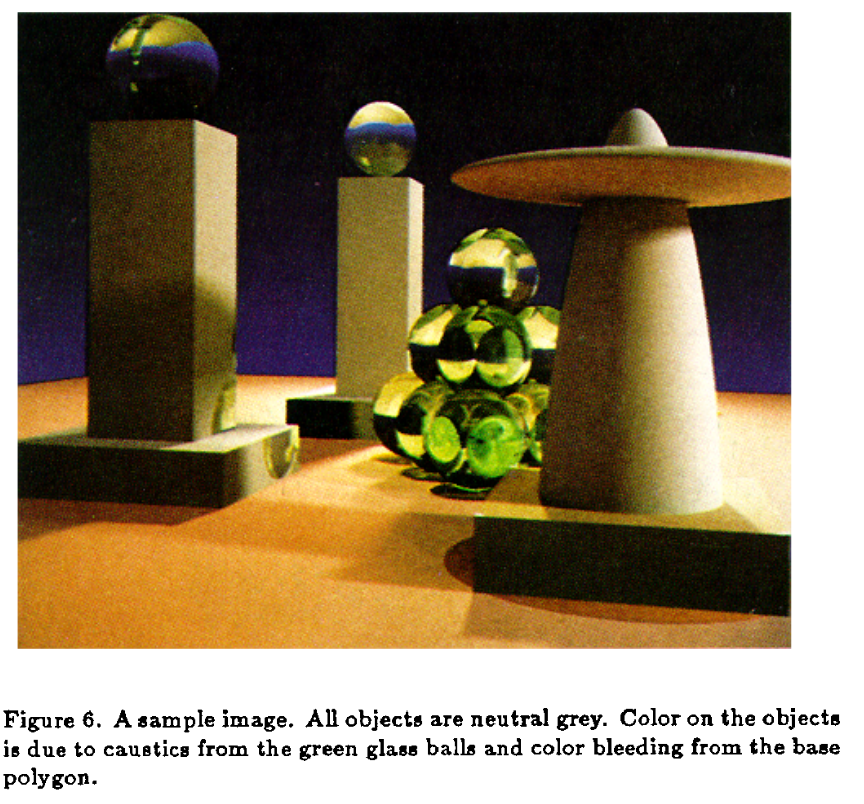
\includegraphics[width=.75\linewidth]{img/1 fundamentals/rendering_eq_figure.png}
	\caption{Figure from \cite{kajiya1986rendering} displaying a scene rendered with his approach.}
	\label{fig:rendering_eq}
\end{figure}


\subsection{Notable Ray Tracing Algorithms}

\section{Solid Representation}

\subsection{Analytical (WT)}

\subsection{Polygon Meshes}

\begin{figure}
	\centering
	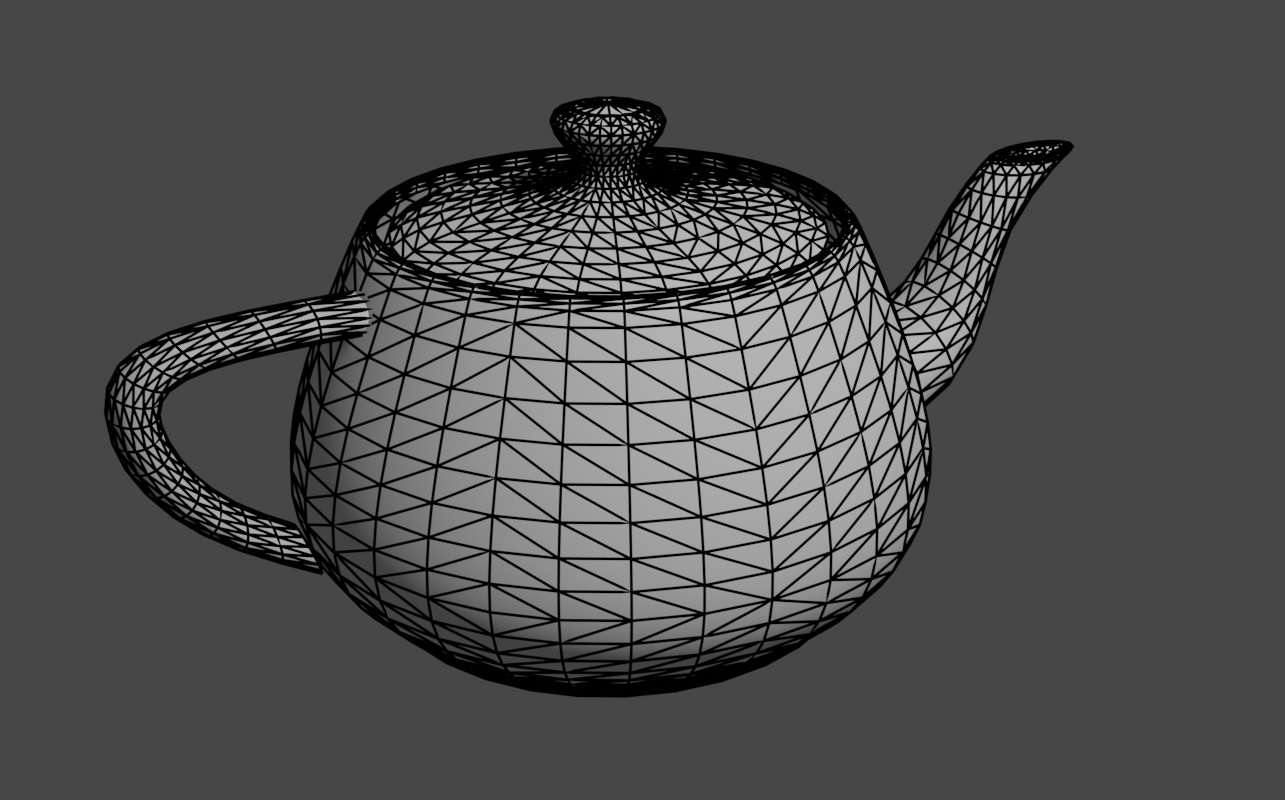
\includegraphics[width=.8\linewidth]{img/1 fundamentals/poly_mesh.png}
	\caption{Polygon mesh of the famous Utah Teapot, rendered with Blender \cite{blender2018}}
	\label{fig:poly_mesh}
\end{figure}

\subsection{Constructive Solid Geometry (CSG)}

\begin{figure}
	\centering
	\subfloat[\texttt{OR} operator.]{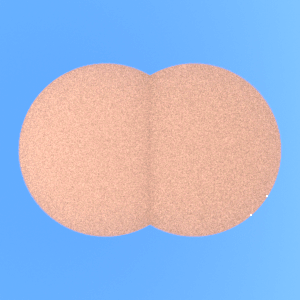
\includegraphics[width=.3\textwidth]{img/1 fundamentals/or.png}\label{fig:csg_or}}
	\hfill
	\subfloat[\texttt{AND} operator.]{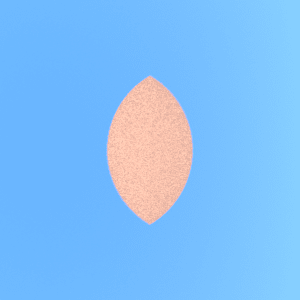
\includegraphics[width=.3\textwidth]{img/1 fundamentals/and.png}\label{fig:csg_and}}
	\hfill
	\subfloat[\texttt{SUB} operator.]{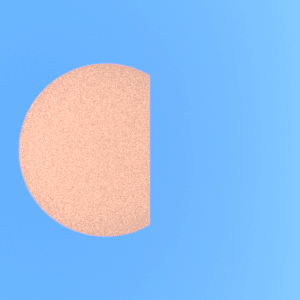
\includegraphics[width=.3\textwidth]{img/1 fundamentals/sub.png}\label{fig:csg_sub}}
	\caption{Boolean operators Union (\ref{fig:csg_or}), Intersection (\ref{fig:csg_and}) and Difference (\ref{fig:csg_sub}) applied to two sphere objects.}
\end{figure}


\begin{figure}
	\centering
	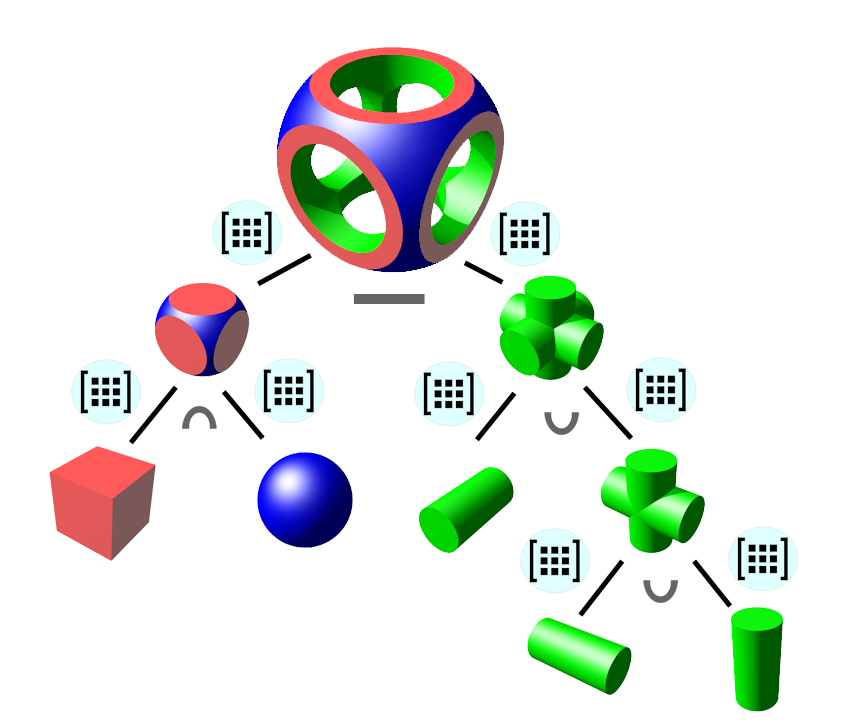
\includegraphics[width=.9\linewidth]{img/1 fundamentals/csg_tree.png}
	\caption{Visualization of a CSG tree hierarchy, originally created by \cite{csgtree} and updated
	with a matrix icon symbolizing affine transformations of geometries.}
	\label{fig:csg_tree}
\end{figure}


\section{Limitations}




% new section
\section{Common ray acceleration data structures}
The computational cost associated with ray tracing algorithms has always been regarded as a "necessary evil" one has to face when desiring highly realistic images. An often cited fact is Whitted's observation, that, for complex scenes, 95 percent of the time used by the algorithm is spend on intersection calculations \cite[p 349]{whitted1979improved}. The image displayed in figure \ref{fig:rendering_eq}, was rendered with a resolution of 512 by 512 pixels and with 40 paths per pixel on an IBM 3081 machine consumed during 1221 minutes \cite[p 149]{kajiya1986rendering}. 

It was a logical consequence, that, over time, new ideas were introduced for accelerating the ray tracing process, mostly by minimizing the number of intersection tests. Nowadays, there exist various ray acceleration structures. In the following, two of these structures are that are commonly used, namely bounding volume hierarchies and binary space partitioning trees are introduced.

\subsection{Bounding volume hierarchy}

\subsection{Binary space partitioning}


\section{Intel\textregistered's Embree Framework}
Embree is a high performance rendering framework, consisting of a collection of kernels and data structures suited for the communication with [insert hardware types]. The latest version of Embree at the time of writing this thesis is 3.13.0.